\documentclass[conference]{IEEEtran}
%\usepackage{graphicx}
\usepackage[dvipdfmx]{graphicx}
%\usepackage{latexsym}
\usepackage{slashbox}
%\usepackage{multirow}
\usepackage{url}
\usepackage{color}
\usepackage{colortbl}
\usepackage{hhline}
\usepackage{flushend}
\usepackage{verbatim}
%\usepackage{hyperref}
\usepackage{enumerate}
\usepackage[sort&compress]{natbib}
\usepackage{subfigure}
\usepackage{framed}
%\usepackage{natbib}

\newcommand{\todo}[1]{{\color{green}{\textbf{TODO: [#1]}}}}
\newcommand{\yasu}[1]{{\color{red}{\textbf{Yasu says: [#1]}}}}
\newcommand{\emad}[1]{{\color{blue}{\textbf{[#1]}}}}
\newcommand{\Emad}[1]{{\color{blue}{\textbf{[#1]}}}}
\newcommand{\revised}[1]{{\color{red}{#1}}}
\newcommand{\para}[1]{{\color{magenta}{\textbf{This paragraph:}}} [#1]}

%\newcommand{\revised}[2]{\marginpar{\fbox{#2}}{\color{red}{#1}}}

\newcommand{\nbf}[1]{
%  \noindent{\textit{\textbf{#1}}}
  \noindent{\textbf{#1}}
}

\newcommand{\conclusionbox}[1]{%
	\vspace{2mm}
  \noindent
	\framebox[0.48\textwidth][c]{%
		\parbox[b]{0.45\textwidth}{%
			{\em #1}
		}
	}
}

% Set bibliography title
%\renewcommand\refname{REFERENCES}
%\renewcommand\bibsection{\section{\refname}}

\newcommand{\ea}{{\em et al.}}
\newcommand{\smallsection}[1]{\vspace{1mm}\noindent {\bf #1}.\hspace{2mm}}
\newcommand{\emphsection}[1]{\vspace{1mm}\noindent \underline{{\em #1}.}\hspace{2mm}}


% Reduce bibliography font size
%\def\bibfont{\normalsize} %normalsize should be default
% small or footnotesize

% Reduce space between references
%\setlength{\bibsep}{3.2pt} %3.5pt should be default


\begin{document}

\title{How Much do We Pay for Technical Debt as Interest?}

\author{
\IEEEauthorblockN{Yasutaka Kamei$^{\dag}$, Everton Maldonado$^{\dag\dag}$, Emad Shihab$^{\dag\dag}$, and Naoyasu Ubayashi$^{\dag}$}
\IEEEauthorblockA{
$^{\dag}$Principles of Software Languages Group (POSL), Kyushu University, Fukuoka, Japan\\
$^{\dag\dag}$Department of Computer Science and Software Engineering, Concordia University, Montr\'eal, Canada\\
Email: $^{\dag}$\{kamei, ubayashi\}@ait.kyushu-u.ac.jp, $^{\dag\dag}$\{e\_silvam, eshihab\}@encs.concordia.ca
}
}

% make the title area
\maketitle

% As a general rule, do not put math, special symbols or citations
% in the abstract
\begin{abstract}
abstract.
\end{abstract}

\IEEEpeerreviewmaketitle

% Here is Yasu't note
\begin{comment}
2 tomato: let's finish results (how to show)
2 tomato: read related work to get knowledge and good motivation for RQ1 and RQ2.

- slide:
2 tomato (one topic of current)
2 tomato (one topic of current)
\end{comment}

%%%%%%%%%%%%%%%%%%%%%%%%%%%%%%%%%%%%%%%%%%%%%%%%%%%%%%%%%%%
%%What is technical debt and self-admitted technical debt
Technical debt is term first coined by Cunningham in 1993 to refer to the phenomena of taking a shortcut to achieve short term development gain at the the cost of increased maintenance effort in the future \cite{Cunningham1992WPM}. The technical debt community, organized through the managing technical debt workshop \cite{Falessi2014MTD}, has studied many aspects of technical debt, including its detection \cite{Zazworka2013CSE}, impact \cite{Zazworka2011MTD}
and the appearance of technical debt in the form of code smells \cite{Fontana2012MTD}. Most recently, we developed an approach to identify technical debt from code comments, referred to as self-admitted technical debt (SATD). SATD refers to the situation where developers know that the current implementation is not optimal and write comments alerting the inadequacy of the solution.

% What people did and what is the impact of TD. What they found.
In the last few years, an increasing amount of work has focused on SATD. In particular, our prior work focused on the detection of SATD~\cite{Potdar2014ICSME} and the classification of different types of SATD and the development of datasets to enable future studies on SATD~\cite{Maldonado2015MTD}. Other work by Bavota and Russo performed an empirical study of SATD on a large number of Apache projects showed that SATD is prevalent in open source projects, is long lived and is increasing over time. A study by Wehaibi et al. \todo{cite Wehaibi} examined the impact of SATD on quality and found that SATD does not necessarily relate to more defects, however, it does make the software system more complex. 

%However, very little work focused on interest. Also, why is calculating interest difficult
Based on these prior findings, we measure and quantify the effect of SATD. In particular, we measure the amount of \emph{interest} caused by SATD. Although the metaphor of technical debt has been well studied, to the best of our knowledge, the quanitification of interest of technical debt has not been examined before. Measuring the interest if technical debt is non-trivial since it requires, in addition to the detection of the technical debt, the tracking of the debt over time and the development of a measure to accurately quantify this debt.

% What we do  and how we calculate interest
In this paper, we first propose the use of code metrics, in particular \todo{add}, as a measure of interest. We 
 
% Main contributions
The main contributions of the paper are three-fold.

\begin{itemize}
\end{itemize}

% Organization of the paper
\smallsection{Paper Organization} To purse the goal of this paper, the paper is organized as follows. 
Section \ref{background} explains the overview of defect prediction models.
Section \ref{past} revisits what challenges were in Year 2000.
%Section \ref{trends} assesses what state the research trend is in.
%Section \ref{game_changers} presents game changers, which dramatically changed perspective and direction of the studies in the field of defect prediction.
Section \ref{trends} assesses what state the research trend is in and presents some of game changers, which dramatically changed perspective and direction of the studies in the field of defect prediction.
Section \ref{challenges} highlights some key challenges for future.
Section \ref{conclusion} draws conclusions.

\section{Introduction}
\para{What is technical debt?}

\para{Describe more detail of technical debt and current problem in the domain}

\para{The goal and approach of this study}

\para{Contributions}

\cite{Potdar2014ICSME}
\cite{Maldonado2015MTD}

%%%%%%%%%%%%%%%%%%%%%%%%%%%%%%%%%%%%%%%%%%%%%%%%%%%%%%%%%%%
%\section{Background} \label{background}
%\emph{Prevention is better than cure.}
\para{Technical debt}

\cite{Guo2011ICSM}: they track technical debt items and access its impact (cost) among incurred, deferred and paid. That said, they focused on only one event (WebDav protocol is not supported) and 

\para{Software Evolution: We calculate interest by looking at the difference size of two versions. In other words, this work is one of lines of software evolution.}
\section{Related Work}
\para{Technical debt}

\cite{Guo2011ICSM}: they track technical debt items and access its impact (cost) among incurred, deferred and paid. That said, they focused on only one event (WebDav protocol is not supported) and 

\para{Software Evolution: We calculate interest by looking at the difference size of two versions. In other words, this work is one of lines of software evolution.}

%%%%%%%%%%%%%%%%%%%%%%%%%%%%%%%%%%%%%%%%%%%%%%%%%%%%%%%%%%%
\section{Case Study Setup}
The goal of this study is \todo{purpose.}.
...

We formalize our study in the following research questions:

\todo{List up research question}

To conduct our case study, we use data from ...

\todo{How do we choose projects we analyze? i.e., why do we use Ant and Jmeter and do not use ArgoUML, Columba and JFreeChart? and why do we add jruby?}

Similar to previous work~\cite{Kamei2010ICSM,Kamei2013TSE}, we used churn as effort. We assume that developers spend their effort to check the method before modifying methods at least, we say that is the effort.

\subsection{Project Data Extraction}
\para{Get Git repos}

\para{}

\subsection{Interest}
To measure interest, we use source code metrics. We use Understand, which is a well-known tool, to measure source code metrics. 

\para{how to calculate metrics?}

In this study, we consider the relative size of ... as interest. For example, 

\para{how to identify when a technical debt are introduced and removed?}
From that version, we obtain patches between two versions over all versions for each file that includes technical debt. Then, we check each patch about whether or not technical debt is introduced/removed. Some of them are not removed. If so, we use latest commits. We calculate the difference of a metric between two versions when technical debt is introduced and removed.

%%%%%%%%%%%%%%%%%%%%%%%%%%%%%%%%%%%%%%%%%%%%%%%%%%%%%%%%%%%
\section{Results}
\subsection{RQ1: Can we quantify interest of technical debt at the function-level?}
\smallsection{Motivation}
\todo{need to read some papers that say technical debt is bad. So we want to quantify it.}

\smallsection{Approach}
\para{We calculate the interest.}

\smallsection{Results}

Put Table.

Figure xx shows that the distribution of interest. X
\para{Put the distribution of interest?}

割合と分布について述べる.

%-----------------------------------------------------------------------
\begin{figure}
  \centering
  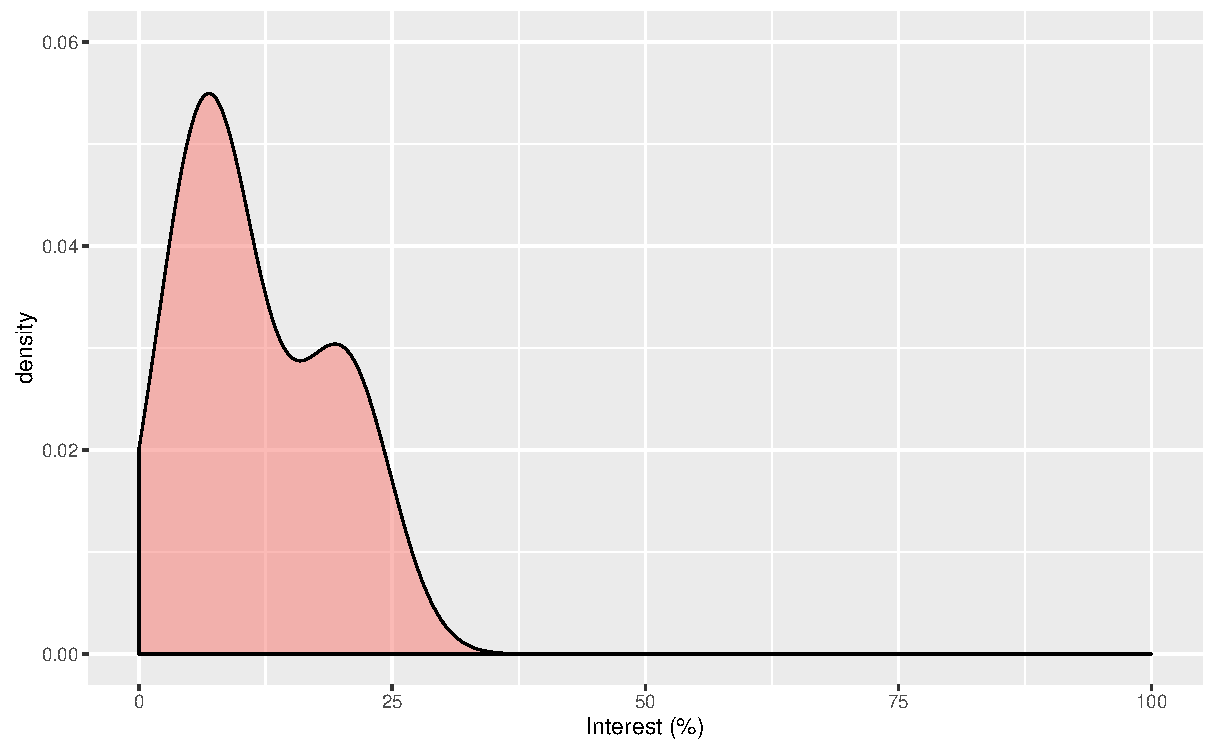
\includegraphics[width=.45\textwidth]{figures/rq1-ant}
  \caption{Adding a Repository in Commit Guru \label{fig:guru1}}
\end{figure}
\begin{figure}
  \centering
  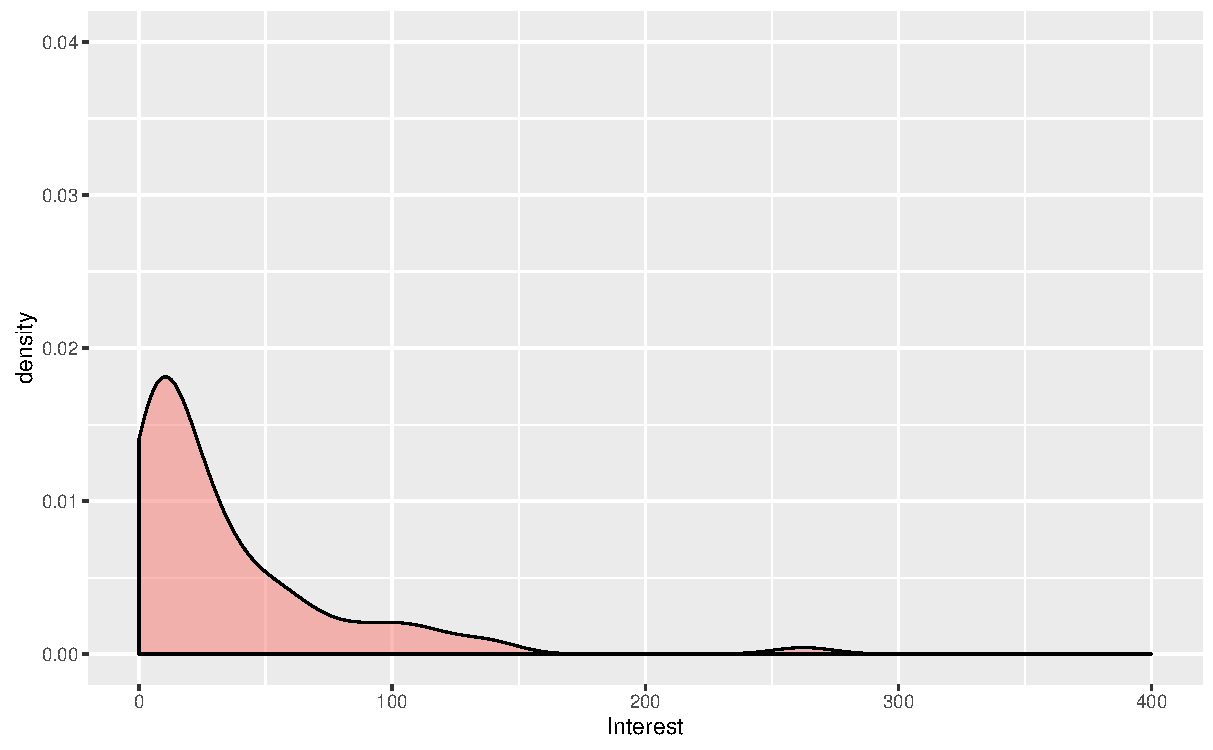
\includegraphics[width=.45\textwidth]{figures/rq1-jmeter}
  \caption{Adding a Repository in Commit Guru \label{fig:guru1}}
\end{figure}
\begin{figure}
  \centering
  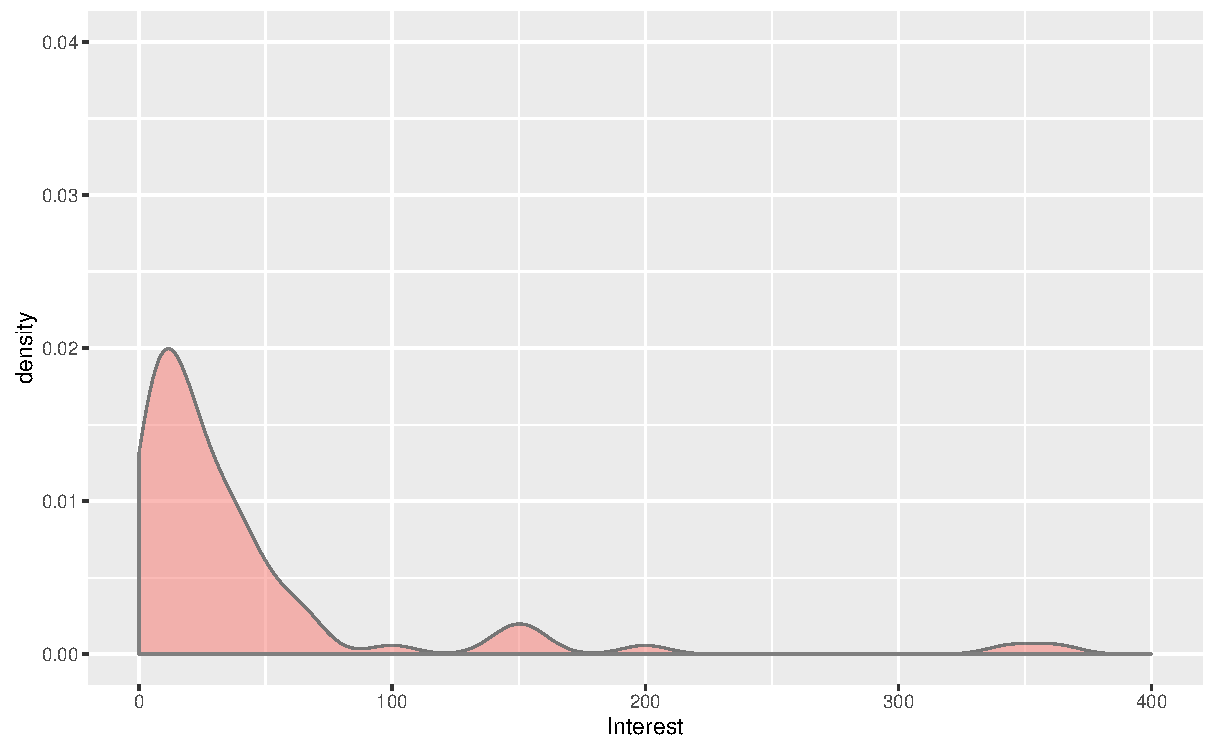
\includegraphics[width=.45\textwidth]{figures/rq1-jruby}
  \caption{Adding a Repository in Commit Guru \label{fig:guru1}}
\end{figure}
%-----------------------------------------------------------------------


\conclusionbox{Result of RQ1: 22\%-36\% of technical debt has positive interest.}

\subsection{RQ2: Does the interest differ based on the type of technical debt?}
\smallsection{Motivation}
There are several type of technical debt such as defect technical debt and design technical debt. 
To better understand the interest, we would like to analayze ...

\smallsection{Approach}
We classify technical debt into categories and calculate interest in each category.

\smallsection{Results}
Table X shows the number and the percentage of technical debt. Among three projects, jruby only includes more than one category that has more than 10\% of technical debt methods. Therefore, we decided to use jruby in RQ2.

\para{we report same things in RQ1.}  

%-----------------------------------------------------------------------
\begin{figure}
  \centering
  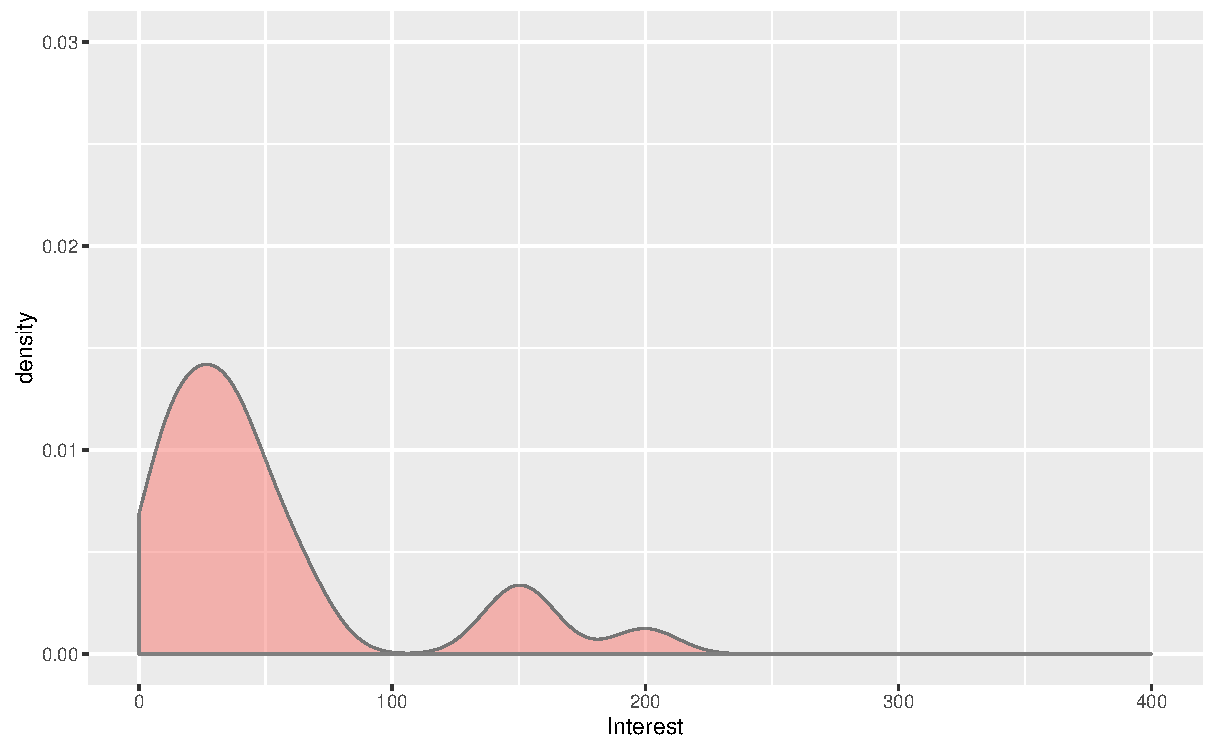
\includegraphics[width=.45\textwidth]{figures/rq2-defect}
  \caption{Adding a Repository in Commit Guru \label{fig:guru1}}
\end{figure}
\begin{figure}
  \centering
  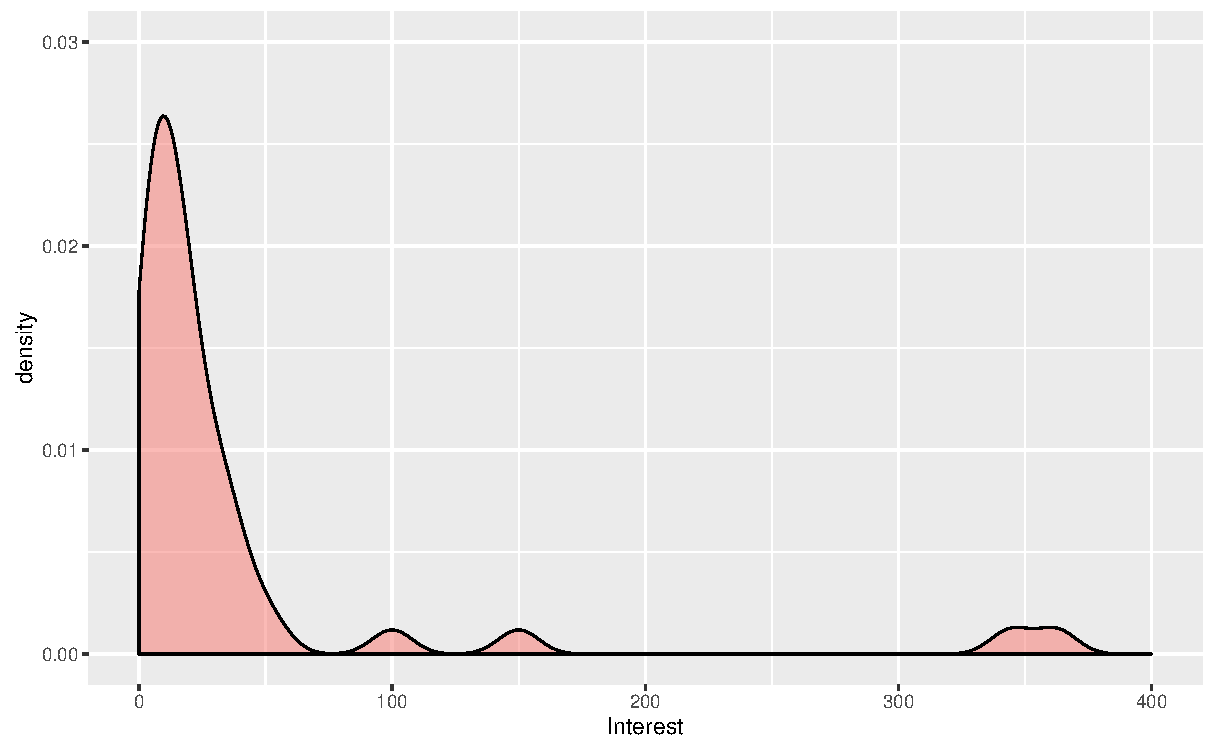
\includegraphics[width=.45\textwidth]{figures/rq2-design}
  \caption{Adding a Repository in Commit Guru \label{fig:guru1}}
\end{figure}
\begin{figure}
  \centering
  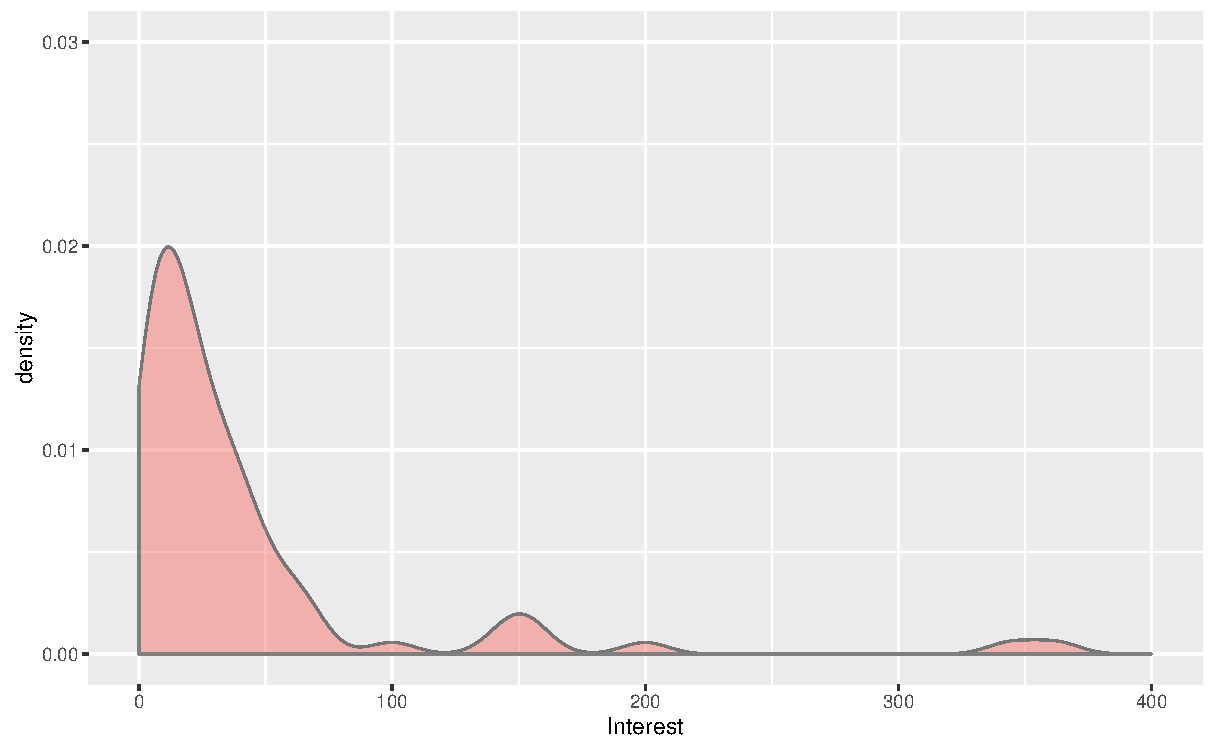
\includegraphics[width=.45\textwidth]{figures/rq2-requirement}
  \caption{Adding a Repository in Commit Guru \label{fig:guru1}}
\end{figure}
%-----------------------------------------------------------------------


\conclusionbox{Result of RQ2}

\subsection{RQ3: manual analysis}
\smallsection{Motivation}

\smallsection{Approach}

\smallsection{Results}

\conclusionbox{Result of RQ3}

\section{Discussion}
\para{Put additional analysis when considering time period.}

\para{Put additional analysis when considering other metrics (fan-in).}

\para{Put additional analysis when comparing the non-technical deb methods.}

\para{Put the analysis for showing the method that includes more than one technical debt in one version.}

%%%%%%%%%%%%%%%%%%%%%%%%%%%%%%%%%%%%%%%%%%%%%%%%%%%%%%%%%%%
\section{Threat to Validity}

\smallsection{Construct Validity}

\smallsection{Internal Validity}
\para{Technical debt is classified by one person.}

\smallsection{External Validity}

%%%%%%%%%%%%%%%%%%%%%%%%%%%%%%%%%%%%%%%%%%%%%%%%%%%%%%%%%%%
\section{Conclusion}
%\section{Conclusion} \label{conclusion}
%\section{Conclusion} \label{conclusion}
%\section{Conclusion} \label{conclusion}
%\input{conclusion.tex}
\para{Summary of this work.}

\smallsection{Future direction}

\begin{itemize}
\item \todo{Discuss how to calculate interest.}
\item  There are several type of technical debt such as defect technical debt and design technical debt.
The previous study~\cite{Maldonado2015MTD} shows that the percentage of technical debt varies depending on the type of technical debt and the studied systems. For example, the projects that have limited time to develop features are likely to leave comments of features that need to be implemented in the future. 
To better understand the interest, we would like to analyze the interest per type of technical debt.
\item  The interest varies among technical debt. If we can understand the reason why some of technical debt has large interest, we can make use of such insights for future development. Therefore, we would like to manually investigate why some of technical debt has large interest.
\item Generally speaking, software systems are always evolving over time for implementing new functionality and fixing defects~\cite{xxx}.
Therefore, even if the size of technical debt increases, it is not clear about how the nature of software evaluation affects the interest of technical debt.
We would like to compare the impact of software evolution on methods in two groups of SATD v.s. non-SATD.
\item To operationalize our findings, we also built a tool that is able to identify and assign an interest rate to all SATD instances in a project. Our tool is publicly available and can be used by practitioners to prioritize the most impacting (i.e., highest interest) SATD.
\end{itemize}

\para{Summary of this work.}

\smallsection{Future direction}

\begin{itemize}
\item \todo{Discuss how to calculate interest.}
\item  There are several type of technical debt such as defect technical debt and design technical debt.
The previous study~\cite{Maldonado2015MTD} shows that the percentage of technical debt varies depending on the type of technical debt and the studied systems. For example, the projects that have limited time to develop features are likely to leave comments of features that need to be implemented in the future. 
To better understand the interest, we would like to analyze the interest per type of technical debt.
\item  The interest varies among technical debt. If we can understand the reason why some of technical debt has large interest, we can make use of such insights for future development. Therefore, we would like to manually investigate why some of technical debt has large interest.
\item Generally speaking, software systems are always evolving over time for implementing new functionality and fixing defects~\cite{xxx}.
Therefore, even if the size of technical debt increases, it is not clear about how the nature of software evaluation affects the interest of technical debt.
We would like to compare the impact of software evolution on methods in two groups of SATD v.s. non-SATD.
\item To operationalize our findings, we also built a tool that is able to identify and assign an interest rate to all SATD instances in a project. Our tool is publicly available and can be used by practitioners to prioritize the most impacting (i.e., highest interest) SATD.
\end{itemize}

\para{Summary of this work.}

\smallsection{Future direction}

\begin{itemize}
\item \todo{Discuss how to calculate interest.}
\item  There are several type of technical debt such as defect technical debt and design technical debt.
The previous study~\cite{Maldonado2015MTD} shows that the percentage of technical debt varies depending on the type of technical debt and the studied systems. For example, the projects that have limited time to develop features are likely to leave comments of features that need to be implemented in the future. 
To better understand the interest, we would like to analyze the interest per type of technical debt.
\item  The interest varies among technical debt. If we can understand the reason why some of technical debt has large interest, we can make use of such insights for future development. Therefore, we would like to manually investigate why some of technical debt has large interest.
\item Generally speaking, software systems are always evolving over time for implementing new functionality and fixing defects~\cite{xxx}.
Therefore, even if the size of technical debt increases, it is not clear about how the nature of software evaluation affects the interest of technical debt.
We would like to compare the impact of software evolution on methods in two groups of SATD v.s. non-SATD.
\item To operationalize our findings, we also built a tool that is able to identify and assign an interest rate to all SATD instances in a project. Our tool is publicly available and can be used by practitioners to prioritize the most impacting (i.e., highest interest) SATD.
\end{itemize}

\para{Summary of this work.}

\section*{Acknowledgment}
This research was partially supported by JSPS KAKENHI Grant Numbers 15H05306.

\bibliographystyle{abbrv}
%\bibliographystyle{IEEEtranN}
\bibliography{reference}


\end{document}

